\documentclass{article}
\usepackage{microtype,graphicx,booktabs,amsmath,amssymb,amsthm,hyperref}
\usepackage[preprint]{icml2026}
\newtheorem{theorem}{Theorem}
\newtheorem{proposition}{Proposition}
\newtheorem{corollary}{Corollary}
\newcommand{\R}{\mathbb{R}}
\newcommand{\norm}[1]{\left\|#1\right\|}
\newcommand{\ip}[2]{\langle #1,#2\rangle}
\newcommand{\A}{\mathcal A}
\icmltitlerunning{Representation and Alignment Uncertainty in Cryo-EM}
\begin{document}
\twocolumn[
\icmltitle{Continuous Audits of Representation and\\Alignment Uncertainty in Cryo-EM}
\begin{icmlauthorlist}\icmlauthor{Fourier Cryo Splats Project}{anon}\end{icmlauthorlist}
\icmlaffiliation{anon}{Fourier Cryo Splats research project}
\icmlcorrespondingauthor{Project repository}{\url{https://github.com/yashpatel5400/fourier-cryo-splats}}
\icmlkeywords{cryo-EM, uncertainty quantification, inverse problems, validation}
\vskip 0.2in]
\printAffiliationsAndNotice{}
\hypersetup{pdftitle={Continuous Audits of Representation and Alignment Uncertainty in Cryo-EM}}
\begin{center}\small Research manuscript under development; not submitted.\end{center}

\begin{abstract}
Uncertainty in a cryogenic electron microscopy (cryo-EM) reconstruction depends on both its representation and its treatment of estimated alignments. We develop a continuous Fourier-slice audit for fixed linear density features, separating a convenient reconstruction model from the class over which uncertainty is assessed. Analytic adjoint integrals, matrix-free optimization, and explicit integration remainders permit an audit outside a Gaussian fitting dictionary. We distinguish deterministic pose errors from a conditional model of independent centered errors with a bounded shared component, and show why independent inference images alone do not establish the latter model. A matched continuous Gaussian-prior interval can share the fixed-pose uniform guarantee, so fixed-pose coverage is not an advantage over that baseline. A frozen study re-estimates local poses and weights on 600 noisy datasets across three acquisition geometries. All 216 procedure/control cells cover their broad targets in 200/200 trials, including the simpler fixed-pose and Gaussian baselines. The three pose-audit procedures always select the no-data fallback; their raw median widths are 642--1,242 times its width. This study exposes conservatism rather than a coverage advantage. Experimental interval centers were observed before fresh noise calibration; density, pose, and covariance assumptions remain unvalidated. This manuscript does not establish experimentally calibrated density coverage or an advantage at near-atomic resolution.
\end{abstract}

\section{Introduction}
The relevant question for an uncertainty method is which claim its interval supports. A shell correlation, a posterior over conformations, and a local density confidence interval have different estimands and sampling assumptions. Modern neural and Gaussian reconstructions can represent detailed densities, but representational flexibility alone does not determine which features are supported by the observations. We study a specified local average or contrast of a homogeneous density, including the effect of uncertainty outside the representation used to fit a pilot.

Two distinctions motivate the method. First, conditioning on a finite reconstruction dictionary removes possible density errors by assumption. An independent-half reconstruction can inherit the same omission. Second, an interval derived for a fixed Fourier-slice design need not remain valid after estimating that design from noisy particles. Separating alignment and inference observations removes one noise dependence, but does not make alignment errors centered conditional on the resulting design.

Our contribution is an implemented continuous Fourier audit and a validation program that exposes these distinctions quantitatively. It specializes established bias-aware inference: the statistical coverage principle, norm duality, and Gaussian ridge representation are not new. The operator-specific work evaluates continuous residual and pose-derivative fields, controls quadrature in real arithmetic, and records when the resulting intervals are informative. The full study retains matched favorable baselines, numerical failures, and no-data fallbacks. A conditional guarantee is kept separate from evidence that its physical assumptions hold.

\section{Related Work and the Uncertainty Target}
Bayesian reconstruction is foundational in cryo-EM \citep{scheres2012}. Posterior ensembles from Gaussian pseudo-atoms \citep{joubert2015}, variational Fourier-slice density uncertainty \citep{ullrich2020}, and likelihood-Hessian soft modes \citep{rangan2024} directly precede our problem. The latter two already distinguish variance from model error and expose density--pose coupling. We compare against a continuous Gaussian prior with the same operator and directional scale rather than treating a weaker discretized prior as decisive evidence.

CryoDRGN \citep{zhong2021} and ab initio neural reconstruction \citep{drgnai2025} address representation learning and structural recovery. Physical heterogeneity is not automatically uncertainty about one homogeneous density. Gaussian representations are also established \citep{chen2021,chen2025,qu2025,shekar2025,gaussianem2026}; their existence is not our novelty claim. Gaussian Fourier kernels provide our initial pilot, while the final audit does not require a Gaussian density dictionary.

Gold-standard halves and noise substitution assess overfitting \citep{schereschen2012,chen2013}; confidence maps test signal significance \citep{beckers2019}; BioEM and independent-particle validation assess image fit \citep{bioem2013,independent2020}. Enhancement confidence can be calibrated against a proxy map \citep{locscale2026}, and conformal methods can cover an exchangeable population of signal--observation pairs \citep{narnhofer2024}. None should be scored as though it promised our fixed-signal density guarantee. The survey in Appendix~\ref{app:survey} separates these targets and identifies unresolved research questions.

Resolving kernels \citep{backusgilbert1968}, optimal recovery \citep{donoho1994}, and honest bias-aware intervals \citep{armstrong2018} supply the statistical foundations. Moment methods can recover collective information without estimating every pose \citep{sharon2020,subspacemom2026}. Therefore, failure of a local pose audit is not an impossibility result for cryo-EM reconstruction.

\section{Model, Feature, and Conditional Design}
For Fourier convention $F(k)=\int\rho(x)e^{-2\pi i k^\top x}\,dx$, write a particle as
\begin{equation}
Y_i(q)=C_i(q)e^{-2\pi i q^\top t_i}F(E_iq)+\epsilon_i(q).
\end{equation}
$E_i$ embeds the detector plane, $C_i$ is the contrast transfer function (CTF), and frequency and shift units are reciprocal. We realify one representative of each conjugate pair. After specified whitening, the conditional nominal model is
\begin{equation}\label{eq:conditionalmodel}
y=\A_0\rho+d+\epsilon,\qquad \epsilon\sim N(0,I),
\end{equation}
where $d$ represents pose or other imaging error. The feature is $t=\ip{\ell}{\rho}$, with a stated coordinate frame and physical smoothing width. We use a Gaussian local average or signed difference of two averages.

Let $H=L^2([-1/2,1/2]^3)$ and let an independent pilot $\rho_0$ define $\delta=\rho-\rho_0$, $\norm\delta_H\le B$. This supported continuous class is different from a finite voxel or Gaussian class. The norm radius is an assumption, not a consequence of a small data residual. The estimator is
\begin{equation}\label{eq:affine}
\widehat t=\ip{\ell}{\rho_0}+w^\top(y-\A_0\rho_0).
\end{equation}
For the basic theorem, the pilot, design, target, noise model, and weights are fixed independently of inference noise. Using consensus poses fitted to the same particles does not satisfy that premise. If separate alignment images determine the design, the theorem can instead be conditioned on those images, provided the inference noise and its processing have the specified conditional law.

\section{Continuous Representation Audit}
Put $h=\ell-\A_0^*w$, $s=\norm w$, and suppose $|w^\top d|\le b_{\rm pose}$. The total bias bound is
\begin{equation}\label{eq:bias}
b=B\norm h_H+b_{\rm pose}.
\end{equation}
Let $q(s,b,\alpha)$ solve
\begin{equation}\label{eq:folded}
\Phi((q-b)/s)-\Phi((-q-b)/s)=1-\alpha
\end{equation}
for $s>0$, and set $q(0,b,\alpha)=b$.

\begin{theorem}[Fixed-design coverage]\label{thm:coverage}
Under Equation~\eqref{eq:conditionalmodel}, with density and nuisance error fixed independently of inference noise, $\widehat t\pm q(s,b,\alpha)$ covers $t$ with probability at least $1-\alpha$, uniformly over the declared density and nuisance class.
\end{theorem}
\begin{proof}
The error is $-\ip{h}{\delta}+w^\top d+w^\top\epsilon$. Its fixed absolute mean is at most $b$, and its Gaussian standard deviation is $s$. Symmetric Gaussian coverage decreases with absolute mean; Equation~\eqref{eq:folded} evaluates its minimum at $b$.
\end{proof}
The theorem is a classical bias-aware construction. A bias chosen adaptively as $b\operatorname{sign}(w^\top\epsilon)$ need not obey its folded-normal conclusion. The sum width $b+z_{1-\alpha/2}s$ handles a bounded adaptive bias when the noise projection itself remains fixed Gaussian, but not arbitrary data-dependent weights.

\subsection{Auditing outside the fitting dictionary}
If a reconstruction space has orthogonal projector $P_S$, a restricted calculation uses only $\norm{P_Sh}$. Orthogonality gives
\begin{equation}\label{eq:omission}
\norm h^2=\norm{P_Sh}^2+\norm{(I-P_S)h}^2.
\end{equation}
The second term is discarded uncertainty, even if the restricted residual is zero. Our audit evaluates the full continuous residual without estimating an omitted density direction from the inference images. It remains conditional on the declared support and norm class.

On the unit cube, $K(v)=\prod_a\operatorname{sinc}(v_a)$. With $c_j=(w_{Rj}+iw_{Ij})C_j/\sigma$ and $f_w(x)=\operatorname{Re}\sum_j c_je^{2\pi i k_j^\top x}$,
\begin{align}\label{eq:sincgram}
\norm{f_w}^2=\tfrac12\operatorname{Re}\sum_{j,l}\{&c_j\overline c_l K(k_j-k_l)\nonumber\\
&+c_jc_lK(k_j+k_l)\}.
\end{align}
Analytic Gaussian target integrals supply the remaining terms of $\norm{\ell-\A_0^*w}^2$. A matrix-free implementation quadratures only this known adjoint field, not the unknown density. Explicit integration remainders accompany primal residuals and dual feasibility. FINUFFT and rounding errors are checked numerically, not enclosed by interval arithmetic (Appendix~\ref{app:continuous}).

\subsection{Design and the continuous Gaussian baseline}
We minimize the convex sum objective
\begin{equation}\label{eq:sumobjective}
z_{1-\alpha/2}\norm w+B\norm{\ell-\A_0^*w}
\end{equation}
before evaluating the sharper folded-normal width. A feasible dual supplies a stopping gap for this objective; it does not establish optimality of the reported folded-normal width. A no-data alternative uses center $\ip{\ell}{\rho_0}$ and half-width $B\norm\ell$. If selected using only design information, both center and width are replaced.

Write $G=\A_0\A_0^*$ and $a=\A_0\ell$. A continuous isonormal Gaussian prior of directional scale $\tau$ gives
\begin{align}
w_\tau&=(G+\tau^{-2}I)^{-1}a,\label{eq:gaussianweights}\\
v_\tau&=\norm{w_\tau}^2+\tau^2\norm{\ell-\A_0^*w_\tau}^2.
\end{align}
White covariance is not trace class on infinite-dimensional $L^2$: this defines joint Gaussian observations and functionals, not an $L^2$-valued random density. It is the continuous ridge/GP comparison naturally associated with the audit.

\begin{proposition}[Fixed-bias Gaussian envelope]\label{prop:normal}
For $z\ge\sqrt3$ and $t\ge0$, $\Pr(|N(t,1)|\le z\sqrt{1+t^2})\ge2\Phi(z)-1$.
\end{proposition}
The proof is in Appendix~\ref{app:proofs}. At $\tau=B$, $z_{1-\alpha/2}\sqrt{v_\tau}$ therefore shares the uniform fixed-pose class guarantee for $\alpha\le2\Phi(-\sqrt3)$. The folded-normal critical value can be shorter; uniform coverage alone is not a distinction from this baseline. We also retain $\tau=B/2$, for which that implication need not hold. A pose-linearized comparator replaces identity noise covariance by $I+JJ^\top$ using the actual continuous pilot Jacobian. It omits nonlinear and unknown-density/pose interactions.

\section{Pose Errors and What Splitting Changes}
For particle $i$, let $D_i:\R^5\to H$ be the first derivative of its weighted adjoint field with respect to scaled rotation/translation error. Its continuous $5\times5$ Gram is obtained by differentiating the sinc kernel. The scalar derivative satisfies
\begin{equation}
\norm{D_i^*\rho}\le c_i:=\norm{D_i^*\rho_0}+B\norm{D_i}_{\rm op}.
\end{equation}
Let $R_2$ be a uniform scalar second-order remainder over the specified error radii, computed by integrated Fourier moment bounds (Appendix~\ref{app:pose}). For arbitrary bounded errors $\norm{u_i}\le r_i$, a deterministic bias bound is $B\norm h+\sum_i r_i c_i+R_2$. This term need not average away as particle count increases.

An alternative model writes $u_i=\mu_i+\xi_i$, with $\norm{\mu_i}\le\eta_i$ and independent centered $\xi_i$ satisfying $\norm{\xi_i}\le r_i$, conditional on the frozen design, weights, density, and pilot. The $\xi_i$ are independent of measurement noise. This is a stronger assumption than a bounded pose radius.

\begin{theorem}[Conditional mixed-pose bound]\label{thm:mixed}
Under this model, the interval centered at Equation~\eqref{eq:affine} with half-width
\begin{align}\label{eq:mixed}
B\norm h+\sum_i\eta_i c_i+R_2\quad\quad\quad\quad\nonumber\\
+\sqrt{2\log(2/\alpha)\left(\norm w^2+\sum_i r_i^2c_i^2\right)}
\end{align}
has coverage at least $1-\alpha$. The remainder is evaluated over radii $r_i+\eta_i$.
\end{theorem}
\begin{proof}
The first-order random scalar for particle $i$ is centered and lies in $[-r_ic_i,r_ic_i]$. Hoeffding's lemma and independence add their sub-Gaussian variance proxies to the Gaussian measurement variance $\norm w^2$. The two-sided Chernoff bound gives the square-root term. Density bias, shared error, and nonlinear remainder are bounded in absolute value and added outside that tail event.
\end{proof}
We use a sub-Gaussian critical value; substituting a Gaussian quantile would require an additional approximation or distributional assumption.

\paragraph{Estimated poses do not establish conditional centering.}
For fixed true poses, a local error $u=\theta-\widehat\theta$ is measurable with respect to a design containing $\widehat\theta$. Hence $E[u\mid\widehat\theta]=u$, not generally zero. Unconditional symmetry does not supply the premise of Theorem~\ref{thm:mixed}. A random latent-pose model or an unconditional analysis of coupled errors and weights needs its own argument. Our estimated-pose use of Equation~\eqref{eq:mixed} is accordingly an empirical plug-in test, not an automatic application of the theorem.

The issue remains with independent inference images. In the phase model $A=s+\sigma_A Z$, $B=s+\sigma_B W$, with independent circular Gaussian noise and $s>0$, let $\widehat\theta=\arg A$. Same-image alignment has mean $E|A|>s$, whereas independent-image alignment has mean $E\operatorname{Re}(e^{-i\widehat\theta}B)=sE\cos\widehat\theta<s$. Their shrinking intervals can converge to zero coverage. This elementary control and a finite-sample invariant comparator are detailed in Appendix~\ref{app:phase}; alignment attenuation and cross-validation are established concerns.

\section{Validation}
We separate three evidence levels: conditional mathematical/numerical checks with supplied inputs; simulations that repeat estimation under a known generator; and experimental-image applications with unverified inputs. The unit of replication is a newly generated dataset or a genuinely independent exposure, not a target, a method, or multiple intervals on the same data.

\subsection{Acquisition geometries and estimands}
We use EMPIAR-10028 (80S ribosome), 10049 (RAG complex), and 10076 (ribosomal assembly intermediates). Their working fields are 482.4, 236.16, and 419.2\,\AA. Density generators use the frozen pilot-registered EMD-2660, EMD-6487, and EMD-8434 maps. The last is one Class A state, not truth for the heterogeneous 10076 stack. Source-group splits, exact selected indices, download records, and input hashes are retained.

The local-refinement study uses 128 particles, frequency radius five, and two broad Gaussian targets of width .07 field. The separate locked-feature study uses radius twelve and twelve features of width 20\,\AA. Band endpoints are 47.2--96.5\,\AA\ and 19.7--40.2\,\AA, respectively. These experiments address coarse features, not near-atomic accuracy. Supplied scalar noise is used in simulations; experimental recalibration is separate.

\subsection{Representation and matched-prior checks}
All twelve original finite-dictionary estimators replay their archived metrics before changing the generator frame. For the central broad 10028 feature, restricted analytic coverage is $4.18\times10^{-5}$ before registration and $3.73\times10^{-14}$ afterwards. Other features improve or worsen; the full table is retained. Continuous/ambient bias checks address the omitted-space mechanism, but conservative coverage of these particular generators does not calibrate the density class.

The matched continuous Gaussian comparison includes all twelve locked features, $\tau\in\{B,B/2\}$, and fixed/linearized-pose models: 48 fits. Both original and registered generators and all declared perturbations are included. Nonconvergence is reported rather than interpreted as an exact posterior. A numerical-only preflight motivated stronger preconditioning for a separate complete rerun; the original incomplete implementation and failed fits remain available. All 48 rerun fits converge. At $\tau=B$, half-width ratios to the fixed-pose audit are 1.341--1.354 on 10028, .994 on 10049, and .999 on 10076. Minimum conditional coverage across all 672 generator/scenario cases is .995970 against the nominal $.995833$ level, including the half-scale prior. These favorable fixed-generator results do not supply a uniform guarantee for the half-scale prior or for estimated poses.
\IfFileExists{tables/continuous-gaussian-v2-main.tex}{\begin{table}[t]
\centering\small
\caption{Matched continuous Gaussian comparison: range over four locked features per stack. $R$ is half-width divided by the original fixed-pose audit width. $C_{\min}$ is minimum analytic coverage across both generator frames and all seven prescribed pose settings. All 48 solves converge; this is conditional supplied-noise coverage, not refitted-pose validation.}
\label{tab:matchedgaussian}
\begin{tabular}{llrrr}
\toprule
Stack & Pose model & $\tau$ & $R$ range & $C_{\min}$ \\
\midrule
10028 & Fixed & 2 & 1.341--1.353 & 1.000 \\
10028 & Linearized & 2 & 1.342--1.354 & 1.000 \\
10028 & Fixed & 1 & 0.874--0.876 & 1.000 \\
10028 & Linearized & 1 & 0.876--0.877 & 1.000 \\
10049 & Fixed & 2 & 0.994--0.994 & 0.996 \\
10049 & Linearized & 2 & 0.994--0.994 & 0.996 \\
10049 & Fixed & 1 & 0.983--0.984 & 0.996 \\
10049 & Linearized & 1 & 0.983--0.984 & 0.996 \\
10076 & Fixed & 2 & 0.999--0.999 & 0.996 \\
10076 & Linearized & 2 & 0.999--0.999 & 0.996 \\
10076 & Fixed & 1 & 0.990--0.990 & 0.996 \\
10076 & Linearized & 1 & 0.990--0.990 & 0.996 \\
\bottomrule
\end{tabular}
\end{table}
}{\paragraph{Execution status.} The complete numerical rerun is still running; its results are not yet included in this working draft.}

\subsection{Re-estimated local poses and weights}
An independent calibration batch contains 128 datasets per geometry. Test batches contain 200 new datasets per geometry. On every replicate, ten fixed Gauss--Newton iterations refine poses against both the oracle reference and the independent pilot; all interval weights are then recomputed. Initial rotations have RMS $2^\circ$ and shifts RMS .5\,\AA\ around truth. Search limits are relative to initialization, not truth. This is a controlled local-refinement pipeline against fixed templates, not repeated ab initio density learning.

Each replicate generates alignment image $Y_A$ and independent inference image $Y_B$. The same fitted design is applied to each, preserving a paired comparison. Nine procedures include folded/sum fixed-pose audits, deterministic pose audit, mixed intervals with shared radii 0/.1, and four Gaussian comparators. The first five retain raw and no-data-fallback results. Each target/procedure has marginal $\alpha=.05$; there is no simultaneous claim over all displayed methods.

The simulation-calibrated joint pose radius is the maximum of 128 dataset-level calibration scores. Under exchangeability with this same generator, template, geometry and optimizer, a new score exceeds it with probability at most $1/129$. Combining this with noise error .04 gives a narrow marginal guarantee for the independent-image deterministic audit. It is known-truth simulation assistance, not experimental pose calibration or a uniform guarantee across new molecules. The mixed-model premise is not asserted for the fitted designs.
All 600 datasets finish without exceptions, and all 12,000 interval-weight solves converge. Every one of the 216 procedure/control cells has raw and selected coverage 200/200, with individual exact 95\% Monte Carlo interval [.9817, 1]. Consequently, this coarse fixed-generator study does not demonstrate undercoverage of any comparator or a coverage advantage for the proposed bounds.

Table~\ref{tab:refittingwidths} shows the failure of practical informativeness. The three pose-audit procedures always select the no-data interval and never exclude zero. Their raw median widths span 642--1,242 times no data; a post-outcome decomposition of every fit attributes 99.31--99.53\% of the raw mixed-zero width to its nonlinear remainder. Fixed-pose and Gaussian intervals have median relative widths .073--.190. They often resolve the central average, whereas contrast sign exclusion is at most .005 for independent inference images. These results do not establish uniform estimated-pose coverage for the simpler procedures.

Median final rotation RMS ranges from 12.0 to 18.5 degrees, compared with the near-truth $2^\circ$ initialization. The coarse noisy local fit thus worsens poses, even with the oracle template. This is a failure of this declared ten-step local refinement, not evidence about a production pose-refinement pipeline. Pose-ball inclusion ranges from .965 to 1 across realized calibration batches; the rank tolerance guarantee averages over calibration batches as well. The pose bounds here audit the recomputed fixed-audit weights; they are not reoptimized for the pose objective.
\begin{table}[t]
\centering\scriptsize
\caption{Local-refinement results: range of median raw half-width/no-data ratios across both targets and templates. All 216 cells have raw and selected coverage 200/200 (individual exact 95\% Monte Carlo interval [.9817, 1]). $^\dagger$Every trial selects the no-data fallback, with relative width 1 and no sign exclusion. Widths are identical for the paired image controls. This tests the declared recipe, not all possible pose-aware estimators.}
\label{tab:refittingwidths}
\begin{tabular}{lrrr}
\toprule
Procedure & 10028 & 10049 & 10076 \\
\midrule
Fixed folded & 0.087--0.107 & 0.113--0.129 & 0.106--0.126 \\
Fixed sum & 0.089--0.109 & 0.118--0.133 & 0.111--0.131 \\
Bounded pose$^\dagger$ & 775--907 & 987--1039 & 651--718 \\
Mixed 0$^\dagger$ & 761--891 & 973--1026 & 642--707 \\
Mixed .1$^\dagger$ & 922--1079 & 1178--1242 & 777--856 \\
GP $B$, fixed & 0.136--0.169 & 0.157--0.190 & 0.152--0.185 \\
GP $B$, pose & 0.136--0.169 & 0.158--0.190 & 0.152--0.185 \\
GP $B/2$, fixed & 0.073--0.090 & 0.088--0.103 & 0.083--0.101 \\
GP $B/2$, pose & 0.073--0.090 & 0.088--0.104 & 0.084--0.101 \\
\bottomrule
\end{tabular}
\end{table}


\subsection{Experimental application and sensitivity}
Twelve estimators and 116 files were locked before acquiring 128 new noise-calibration exposures per stack. The inference centers had already been observed. Under a common Gaussian covariance model, the raw calibration excludes zero for six fixed-pose features, four with shifts alone, and none with rotation budgets. A later centered calibration changes these counts to ten, six, and zero. It also produces five disagreements with the registered 10076 Class A reference; these are not truth-coverage labels for its heterogeneous particles.

All 96 combinations of feature, pose class, and raw/centered calibration are retained in a fixed-weight breakdown analysis. At the one-degree class, every recorded fixed-weight bias bound already exceeds its observed center even at zero measurement SD. The four centered fixed-pose 10028 density-radius breakdowns span 2.877--4.868 against the declared $B=2$; two 10049 features do not exclude zero even at $B=0$. These conditional sensitivities do not validate the scale, density radius, or noise transfer assumptions. More optimized historical cubic designs improve a selected bound modestly; all five experimental cubic designs still include zero.

\subsection{Computation and reconstruction context}
A separate 10,000-particle quadratic audit completes in 4,965 seconds with 1.95 GB peak resident memory. This establishes that audit's scaling, not high-resolution reconstruction speed or convergence of every pose optimizer. Source snapshots, convergence diagnostics, paired replicate arrays, and failed attempts accompany the results.

Supplied-pose Gaussian, voxel and stock-neural fits, three unknown-pose RELION runs, and original-code CryoLike scores provide reconstruction/prediction context. Their FSCs and image scores are not density coverage. The registered-reference mean FSCs for the three RELION runs are .702, .202 and .122; the last uses a heterogeneous stack against one state. Sampled-resolution censoring, map registration, masks and tuning choices are recorded separately (Appendix~\ref{app:experiments}). We do not claim performance comparable to a full high-resolution production reconstruction from these restricted studies.

\section{Discussion and Limits}
The continuous audit tests a representation omission that a restricted model can hide. Its matched Gaussian comparison also shows where an apparent distinction disappears: at equal operator and directional scale, conventional Gaussian uncertainty can share the fixed-pose guarantee. The substantive question is therefore nuisance treatment and the credibility of the assumed class, rather than whether one estimator is called Bayesian or frequentist.

Estimated alignments change the inference problem. Conditional centered-error bounds can be informative under their model, but independent inference images alone do not validate that model. The end-to-end study measures the resulting procedure and finds that its proposed pose bounds are vacuous. Large nonlinear remainders dominate; the broad targets and conservative fixed-pose baselines leave no demonstrated coverage advantage. This is a failure of the tested construction, not an impossibility theorem for pose-aware inference. No numerical or empirical result here establishes a useful experimental density interval without the stated unverified noise, pose, support, homogeneity and density-energy conditions.

CTF and amplitude uncertainty, particle selection, motion/dose variation, detector correlations, and learned-prior dependence remain material. Experimental 10076 results are stress evidence, not a homogeneous-density validation. Ordinary floating-point calculations with analytic integration control are not fully validated arithmetic. The work remains a research manuscript; numerical tests and model reviews do not establish conference acceptance.

\section*{Reproducibility and Impact}
The public repository preserves protocols, code, hashes, complete outcomes, failures, and earlier manuscript versions. The requested independent reviews and responses are available with their unchanged verdicts. Experimental maps should not be interpreted biologically from an uncalibrated interval or internal agreement alone. The purpose of the audit is to make the assumptions and remaining uncertainty inspectable.

\clearpage
\bibliography{references,uncertainty-references,survey-references}
\bibliographystyle{icml2026}
\clearpage
\appendix
\section{Statistical Identities and Scope}\label{app:proofs}
\subsection{Normal envelope and continuous Gaussian comparison}
Here is a proof of Proposition~\ref{prop:normal}. Write $q(t)=z\sqrt{1+t^2}$ and
$F(t)=\Phi(q(t)-t)+\Phi(q(t)+t)-1$. For $t>0$, set
$c=q'(t)=zt/\sqrt{1+t^2}$. Direct differentiation gives
\[
F'(t)=\phi(q-t)\{(c-1)+(c+1)e^{-2qt}\}.
\]
For $c\ge1$ this is nonnegative. For $0<c<1$, nonnegativity is equivalent to
\[
\operatorname{arctanh}(c)\ge qt=\frac{c}{1-c^2/z^2}.
\]
The absolutely convergent power series have coefficients $1/(2j+1)$ and
$z^{-2j}$, respectively. Since $z^2\ge3$ and $3^j\ge2j+1$ for all
integers $j\ge0$, the inequality holds termwise. Thus $F$ is nondecreasing
and $F(t)\ge F(0)=2\Phi(z)-1$. Symmetry handles negative mean; zero variance
follows directly. This is a sufficient range of $z$, not a claim that
$\sqrt3$ is the sharp boundary.

For $G=\A\A^*$, $a=\A\ell$, $L=\norm\ell^2$, and fixed positive covariance
$\Sigma$, completing a quadratic yields
\begin{align}
v(w)&=w^\top\Sigma w+\tau^2\norm{\ell-\A^*w}^2,\\
w_*&=(G+\Sigma/\tau^2)^{-1}a,\\
v(w_*)&=\tau^2(L-a^\top w_*).
\end{align}
These are the joint Gaussian conditional mean weights and variance for an
isonormal prior. With $\Sigma=I$, $\tau=B$, and fixed weights, the worst
absolute class bias is $b=B\norm{\ell-\A^*w}$. The proposition implies
$z\sqrt{v(w)}$ covers every allowed fixed density at level $1-\alpha$ for
$z=z_{1-\alpha/2}\ge\sqrt3$. The statement even holds for nonoptimal fixed
$w$ if the variance expression on the first line is used. That expression
must not be relabeled the exact posterior variance at an unfinished solve.
The implication does not require drawing a density from the Gaussian prior.
Conversely, posterior calibration averaged over a prior and fixed-density
uniform calibration are different statements in general. The matched result
here prevents claiming that their distinction alone favors our audit.

An isonormal process $W(f)$ has covariance $E[W(f)W(g)]=\ip f g$ for
$f,g\in H$. Joint Gaussian laws of $W(\ell)$ and finitely many observation
functionals exist. Identity covariance on infinite-dimensional $H$ has
infinite trace, so there is no associated finite-energy random element of
$H$ with that covariance. This is a generalized-process comparison, not a
claim that all prior draws belong to the bounded density class.

\subsection{Optimization, duality, and numerical error}
The sum-width problem has dual
\begin{equation}
\min_w z\norm w+B\norm{\ell-\A^*w}
=\max_{\norm v\le B,\,\norm{\A v}\le z}\ip\ell v.
\end{equation}
Express the residual norm as the support function of the radius-$B$ ball.
Minimizing $z\norm w-w^\top\A v$ gives zero when $\norm{\A v}\le z$
and minus infinity otherwise. The continuous norm objective and finite
observation space satisfy the usual convex duality qualification. A simple
feasible certificate is $v=th$ with $h=\ell-\A^*w$ and
$t=\min(B/\norm h,z/\norm{\A h})$, interpreting a zero denominator as
no constraint. It gives lower bound $t(L-w^\top a)$. We report the gap for
this sum objective; selecting a folded-normal width afterwards does not
make that width globally optimal.

For $H_\tau=G+\Sigma/\tau^2$ and residual $r=H_\tau w-a$, completing the
same quadratic gives
\begin{equation}\label{eq:solvegap}
v(w)-v(w_*)=\tau^2r^\top H_\tau^{-1}r.
\end{equation}
If $FF^\top\preceq G$ is a truncated pivoted-Cholesky approximation and
$\Sigma\succeq I$, put $P=FF^\top+I/\tau^2$. Then
$P\preceq H_\tau$ and the right-hand side is at most
$\tau^2r^\top P^{-1}r$. Adding a residual diagonal to this preconditioner
need not preserve this ordering. If an approximate Gram action has residual
error at most $e$, then
\[
\sqrt{r^\top P^{-1}r}\le
\sqrt{r_Q^\top P^{-1}r_Q}+\tau e.
\]
We use this as a numerical optimization diagnostic, with the analytic
integration remainder below. Roundoff and transform approximation are not
validated enclosures, and a small variance gap alone does not bound mean
error for every possible observed image vector.

\section{Continuous Fourier Computation}\label{app:continuous}
\subsection{Adjoint and target integrals}
Integrating the two conjugate expansions of a real Fourier field yields
Equation~\eqref{eq:sincgram}. For a unit-mass Gaussian component of center
$\mu$ and standard deviation $\sigma_\ell$, its one-dimensional transform
truncated to the unit interval is
\begin{align}
&e^{-2\pi i k\mu-2\pi^2\sigma_\ell^2k^2}\nonumber\\
&\quad\times[\Phi((1/2-\mu)/\sigma_\ell+2\pi i\sigma_\ell k)\nonumber\\
&\hspace{45pt}-\Phi((-1/2-\mu)/\sigma_\ell+2\pi i\sigma_\ell k)].
\end{align}
Products over coordinates and linear combinations over target components
give $\A\ell$. Gaussian-product integrals give $\norm\ell^2$. The sign
of the transform follows the convention in the main text. Independent
tensor quadrature and a conic formulation using the joint Hilbert Gram of
$[\ell,\A_1^*,\ldots,\A_m^*]$ check these expressions and the optimizer.

For $r$ Gauss--Legendre nodes on a unit interval, let
\[
C_r=\frac{(r!)^4}{(2r+1)((2r)!)^3},\quad
E_r=\sum_{a=1}^3 C_r(4\pi M_a)^{2r},\quad
M_a=\max_j|k_{ja}|.
\]
The classical derivative remainder \citep{dlmfquadrature} gives, for the
positive tensor weights $\omega_t$,
\begin{equation}
\left|\norm{f_w}^2-\sum_t\omega_t f_w(x_t)^2\right|
\le E_r\left(\sum_j|c_j|\right)^2.
\end{equation}
Indeed, the exponential expansion of $f_w^2$ has coordinate frequencies at
most $2M_a$ and coefficient absolute sum at most $(\sum_j|c_j|)^2$.
Apply the one-dimensional remainder in each coordinate and telescope the
three integration/quadrature operators; their positive weights sum to one.
Likewise,
\begin{equation}
\norm{(G-G_Q)w}\le\sqrt2 E_r\norm{C/\sigma}_2\sum_j|c_j|.
\end{equation}
We add the scalar error to the squared residual and the vector error to the
dual feasibility denominator. This preserves a continuous primal/dual
bracket in real arithmetic. At radius five, order 40 gives a kernel
remainder no larger than $3.21\times10^{-23}$ before coefficient scaling.
Two type-3 transforms apply $G_Q$. Requested FINUFFT tolerance $10^{-12}$ is
checked against independent sinc Grams; it is not a rigorous floating-point
bound. Cached plans change setup overhead, not the mathematical operator.

\subsection{Constant-cell generators and spectral Gaussian pilots}
An orthonormal constant-cell coefficient has density value $d^{3/2}$ on a
cell of volume $d^{-3}$. Its transform includes the exact cell sinc product
$\prod_a\operatorname{sinc}(k_a/d)$ and the half-cell phase relative to a
centered FFT grid. Target coefficients use Gaussian CDF differences. Thus
a piecewise constant simulation density is projected as a continuous
function, not as point samples. Generator grids of 64 and pilot grids of
24 have the same continuous norm convention; unit-normalizing both makes
$B=2$ sufficient by the triangle inequality. It does not calibrate an
experimental density-energy radius.

The original fitting representation is a Hermitian sum of Gaussian Fourier
kernels. A kernel away from zero frequency has an oscillatory spatial
counterpart; a shifted real-space Gaussian instead contributes a phase ramp
to a zero-centered Fourier envelope. They should not be conflated. In the
present study the Fourier-Gaussian fit supplies a pilot and reconstruction
baseline. The continuous audit allows density directions outside that
finite representation. Gaussian representations and analytic projection
are prior art, not a novelty claim of the uncertainty construction.

\section{Pose Derivatives, Remainders, and Calibration}\label{app:pose}
\subsection{First derivative and second-order control}
For each particle write $c_{iq}=(w_{R,iq}+iw_{I,iq})C_{iq}/\sigma$.
Use a rotation scale $a$ in radians, detector translation scale $s_t$ in
field units, and dimensionless local error $u\in\R^5$. Its rotation is
$\exp(a[u_{1:3}]_\times)$ and translation $s_tu_{4:5}$. The five
first-adjoint derivatives are real polynomial Fourier fields: rotation
columns have polynomial $2\pi i a\,c_{iq}(k_{iq}\times e_j)^\top x$;
translation columns have $2\pi i s_t c_{iq}q_j$. The sign convention
matches the implemented dephasing and is checked by finite differences.

Their $5\times5$ Hilbert Gram follows from integrals of
$[1,x,y,z][1,x,y,z]^\top e^{2\pi i v^\top x}$ at both frequency sums and
differences. These integrals are derivatives of $K(v)$. The square root
of the largest Gram eigenvalue gives $\norm{D_i}_{\rm op}$. A small
cancellation pad is a floating-point diagnostic, not a proved rounding
bound. The pilot derivative pairing is integrated using the same exact
constant-cell representation.

For a unit vector $b$ and $x$ uniform on the cube,
$E(b^\top x)^2=1/12$ and $E(b^\top x)^4\le13/720$. Along a unit pose
segment the phase derivative consequently satisfies
\begin{align}
\norm{\phi'}_4&\le L_{4,iq}
=2\pi\{a\norm{k_{iq}}(13/720)^{1/4}+s_t\norm{q_{iq}}\},\\
\norm{\phi''}_2&\le H_{2,iq}=2\pi a^2\norm{k_{iq}}/\sqrt{12}.
\end{align}
Since $(e^{i\phi})''=e^{i\phi}(i\phi''-(\phi')^2)$, Minkowski and
H\"older give a second derivative norm at most $H_{2,iq}+L_{4,iq}^2$.
Writing $P_0=\norm{\rho_0}$, Taylor's integral remainder and
Cauchy--Schwarz yield the uniform scalar bound
\begin{equation}\label{eq:secondremainder}
R_2=\frac{B+P_0}{2}\sum_i (r_i+\eta_i)^2
\sum_q|c_{iq}|(L_{4,iq}^2+H_{2,iq}).
\end{equation}
This bound remains valid for large prescribed radii but can become useless.
It retains all second-order and higher effects through the exact derivative
bound along the segment; it is not a second-order truncation without a
remainder. Triangle bounds lose possible cancellation and are not claimed
sharp. The mixed-pose theorem follows by combining this remainder with
Hoeffding's lemma as in the main text.

The historical quadratic/cubic audits retain shared density fields across
particles and add higher-order integration-controlled remainders. Their
complete code, proofs, failed optimizers, and outcomes remain in the
repository. They are not substituted into the frozen local-refinement
experiment after seeing its results.

\subsection{Simulation-assisted maximum-score calibration}
Let $S_1,\ldots,S_m,S_{m+1}$ be exchangeable dataset scores for one fixed
truth, geometry, optimizer, and template. Rank symmetry, with random
tie-breaking if needed, gives
\[
\Pr\{S_{m+1}>\max_{j\le m}S_j\}\le1/(m+1).
\]
The score here is the maximum over particles of
$\sqrt{(\text{angle in degrees})^2+(\text{shift in \AA}/0.5)^2}$.
For $m=128$, its maximum determines a joint rotation/shift ball for the
next dataset. On that event, the deterministic bound with independent
inference images has conditional noise error at most .04. Union with the
score failure yields unconditional error at most $.04+1/129<.05$.
This averages over calibration as well as test datasets. It is not a
conditional guarantee for every realized calibration batch. The pilot and
truth are fixed; it is not distribution-free across new molecules or an
experimentally learned pose-confidence ball. Same-image inference lacks
the required conditional noise law.

\section{Phase Alignment Diagnostic}\label{app:phase}
\subsection{Bias after same-image and independent-image alignment}
Let $A_j=se^{i\theta_j}+\sigma(Z_{1j}+iZ_{2j})$ and
$B_j=se^{i\theta_j}+\sigma(W_{1j}+iW_{2j})$, with all real coordinates
independent standard normal, fixed $s>0$, and arbitrary fixed true phases.
Set $\widehat\theta_j=\arg A_j$. Rotational symmetry reduces the mean
calculation to $\theta_j=0$. Strict Jensen inequality for the norm gives
$E|A_j|>s$. Independence gives
$E\operatorname{Re}(e^{-i\widehat\theta_j}B_j)
=sE\cos\widehat\theta_j<s$ when $\sigma>0$.
Both errors persist as more particles are independently aligned. The law
of large numbers and any half-width tending to zero imply coverage of $s$
tends to zero. Estimating the aligned observations' sampling variance does
not remove their bias. This elementary control diagnoses the mechanism;
it is not an impossibility theorem for marginalized or invariant inference.

\subsection{Invariant comparison with a finite-sample bound}
Put $X_j=\operatorname{Re}(\overline A_jB_j)$ and $m=s^2$.
Then $EX_j=m$ and $\operatorname{Var}(X_j)=2(\sigma^4+m\sigma^2)$.
A product-normal Gaussian integral, or the difference of independent
noncentral and central chi-squares, gives for $|t|<1/\sigma^2$
\begin{equation}
\log E e^{t(X_j-m)}=-\log(1-\sigma^4t^2)
+\frac{m\sigma^2t^2}{1-\sigma^2t}.
\end{equation}
For verification, take real two-vectors $U=(A+B)/(\sqrt2\sigma)$ and
$V=(A-B)/(\sqrt2\sigma)$; their squared norms have two-degree chi-square
laws, with noncentrality $2m/\sigma^2$ for $U$. Since
$X=(\sigma^2/2)(\norm U^2-\norm V^2)$, the displayed expression follows.
For either sign of $t$, the centered log MGF is bounded by
$(\sigma^4+m\sigma^2)t^2/(1-\sigma^2|t|)$. The independent-sum Chernoff
bound with $x=\log(2/\alpha)$ implies
\begin{equation}
\Pr\left\{|\overline X-m|>
2\sqrt{(\sigma^4+m\sigma^2)x/n}+\sigma^2x/n\right\}\le\alpha.
\end{equation}
Invert over $m\ge0$ and square-root endpoints to obtain a confidence set
for $s$. Empty sets are saved as empty, not converted to $[0,0]$.
The guarantee requires known equal Gaussian coordinate noise and identical
signal across the pair; motion, dose, CTF error and heterogeneous amplitudes
would require a different analysis. This is an elementary concentration
specialization and a classical invariant control, not new cryo-EM theory.

\begin{figure*}[t]
\centering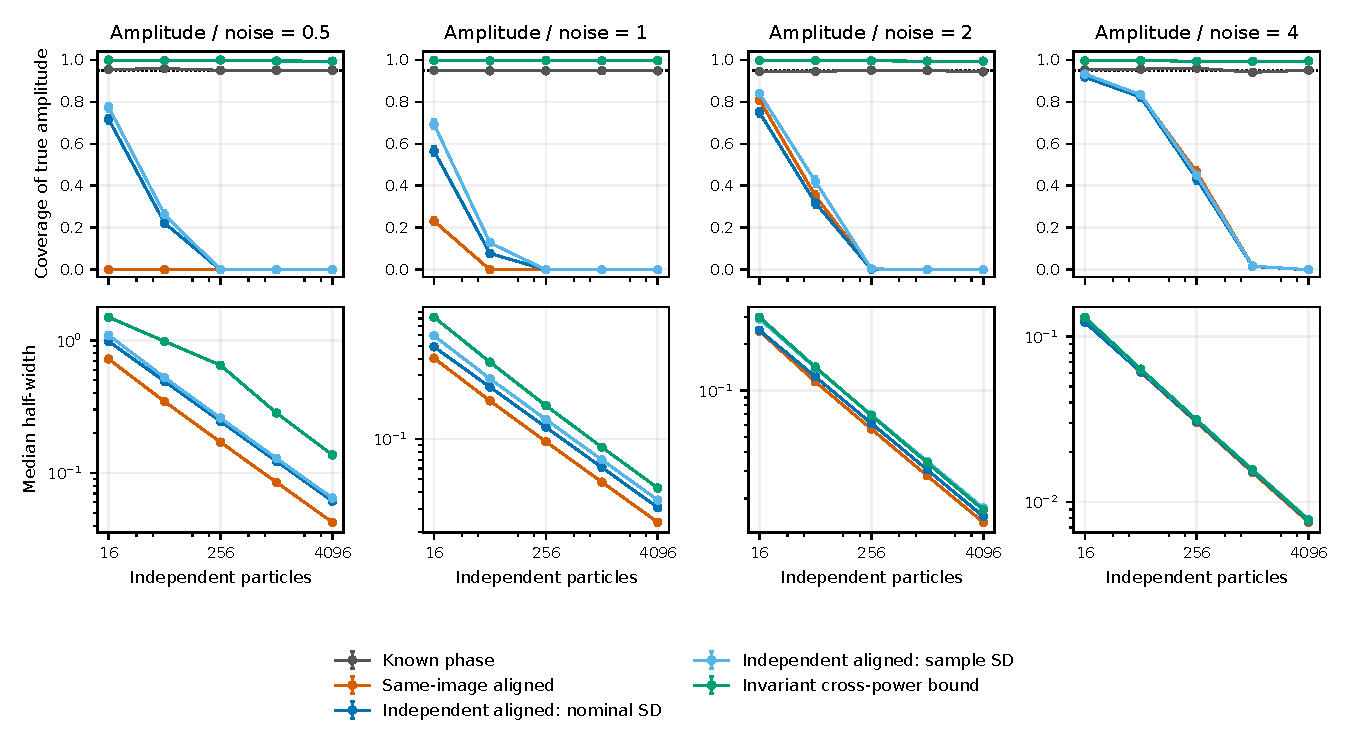
\includegraphics[width=\textwidth]{figures/phase-split-control.pdf}
\caption{Declared phase-only control: 2,000 independent datasets per case,
five paired procedures, four amplitude-to-coordinate-noise ratios, and five
particle counts. At 4,096 particles all three naive aligned intervals have
zero observed coverage in every noise setting. Independent-image sample
variance does not correct attenuation. Oracle coverage is near .95; the
invariant concentration interval is conservative. Width and coverage are
both retained. This is a one-frequency mechanism diagnostic with known
noise, not a reconstruction benchmark.}
\label{fig:phasecontrol}
\end{figure*}

\section{Experimental Protocols and Complete Reporting}\label{app:experiments}
\subsection{Data provenance and independence}
The project downloads experimental particles and metadata from EMPIAR and
reference maps from EMDB. Exact URLs, selected indices, file hashes, signs,
physical fields and software versions accompany each artifact. EMPIAR-10028,
10049 and 10076 supply three distinct acquisition geometries, not three
independent repetitions of a molecular population. Reference maps are
approximate external structures used as simulation generators and agreement
comparators. Pilot-only frame/hand registration is frozen before the
registered replay; the same maps in their original frame remain reported.
Registration does not turn a map into experimental ground truth.

Particle splits use acquisition groups. Within the existing particle
cohorts, poses and CTF metadata may derive from full-data processing; a
particle split does not undo this dependence. The noise-calibration
experiment acquires 128 additional exposures per stack after locking the
estimators and 116 calibration-related files. Its density interval centers
had already been inspected, and the common covariance and transfer
assumptions remain unverified. Selection of the three pilot regions and
matched center precedes those fresh calibration images, but the full
project is development research rather than a prospectively blinded
experimental confirmation.

EMPIAR-10076 contains assembly intermediates. A homogeneous simulation
using registered EMD-8434 Class A is a legitimate fixed-generator test but
is not ground truth for its heterogeneous experimental stack. All biological
interpretations of those experimental consensus features retain this limit.

\subsection{Registered representation replay}
The twelve original dictionary examples use two targets and two widths on
each geometry. Existing weights exactly replay their archived widths, biases
and analytic coverages before the reference frame is changed; the maximum
stored discrepancy is zero. Native versus two-stage resampling changes the
original generator's projections by at most $2.15\times10^{-7}$ relatively.
There is no refit to favor the registered comparison.
\IfFileExists{tables/registered-dictionary-replay.tex}{\begin{table}[t]
\centering\small
\caption{All registered dictionary replays. Coverage is analytic under the supplied fixed design/noise. Ambient-audited coverage is numerically one in both frames for these generators; this is not experimental density coverage.}
\begin{tabular}{llrrr}
\toprule
Stack & Target & SD/field & Original & Registered \\
\midrule
10028 & Center & 0.03 & 0 & 0 \\
10028 & Contrast & 0.03 & 0.916 & 0.054 \\
10028 & Center & 0.07 & $4.18\times10^{-5}$ & $3.73\times10^{-14}$ \\
10028 & Contrast & 0.07 & 0.800 & 0.367 \\
10049 & Center & 0.03 & 0.814 & 0.759 \\
10049 & Contrast & 0.03 & 0.002 & 0.507 \\
10049 & Center & 0.07 & 0.871 & 0.928 \\
10049 & Contrast & 0.07 & $4.90\times10^{-16}$ & 0.786 \\
10076 & Center & 0.03 & 0.001 & 0.250 \\
10076 & Contrast & 0.03 & 0.605 & 0.380 \\
10076 & Center & 0.07 & 0.918 & 0.942 \\
10076 & Contrast & 0.07 & 0.670 & 0.899 \\
\bottomrule
\end{tabular}
\end{table}
}{}
The finite ambient audit and the continuous audit concern different declared
spaces. Both illustrate representation sensitivity, but an ambient-voxel
result is not relabeled a continuous theorem. Near-unit coverage on a
particular generator can coexist with wide or biologically unhelpful intervals.

\subsection{Matched continuous Gaussian comparison}
The frozen comparison has 128 particles per geometry, frequency radius 12,
geometry seed 609315, order-80 quadrature, and 20\,\AA\ targets. It uses the
same twelve pilot-locked locations as the continuous audit, $B=2$, prior
scales 2 and 1, and $\alpha=.05/12$. Fixed-pose covariance is identity after
supplied whitening. The local-Gaussian alternative uses the actual
continuous pilot Jacobian, with coordinate SDs $1^\circ$ and .5\,\AA.
This is a first-order working model, not the bounded nonlinear pose class.

For each of 48 fits, both original and registered generators are projected
at nominal poses and at all six declared perturbations: rotation scales
0, 1 and 2 degrees, each with coherent and random-boundary directions and
translation scale .5\,\AA. The zero-degree perturbation setting can still
include shifts and differs from the nominal case. Conditional fixed-signal
coverage and correct-sign probability are computed from their exact scalar
Gaussian laws under the supplied noise. These are not end-to-end coverage
experiments. All 672 fit/frame/scenario evaluations are retained.

The initial rank-1,024 implementation was interrupted after four fits, all
nonconverged at the 2,000-iteration limit. Its first residual was about
$1.04\times10^{-5}$ and a residual-based variance-gap diagnostic was about
9\%. Its JSON, weights, logs and incomplete flag are preserved. A numerical
preflight, without new pixels or coverage selection, increased the
preconditioner rank to 8,192: after 315 seconds of setup, the first system
reached residual $9.50\times10^{-12}$ in three warm-started iterations.
The declared complete rerun uses this rank, cached transforms, zero initial
weights, one CPU thread, the same $10^{-10}$ tolerance and 2,000-iteration
ceiling, and unchanged scientific settings. All convergence flags and
variance-identity errors remain visible. This amendment is computational,
not a replacement of an unfavorable statistical baseline.
\IfFileExists{tables/continuous-gaussian-v2-detail.tex}{\begin{figure*}[t]
\centering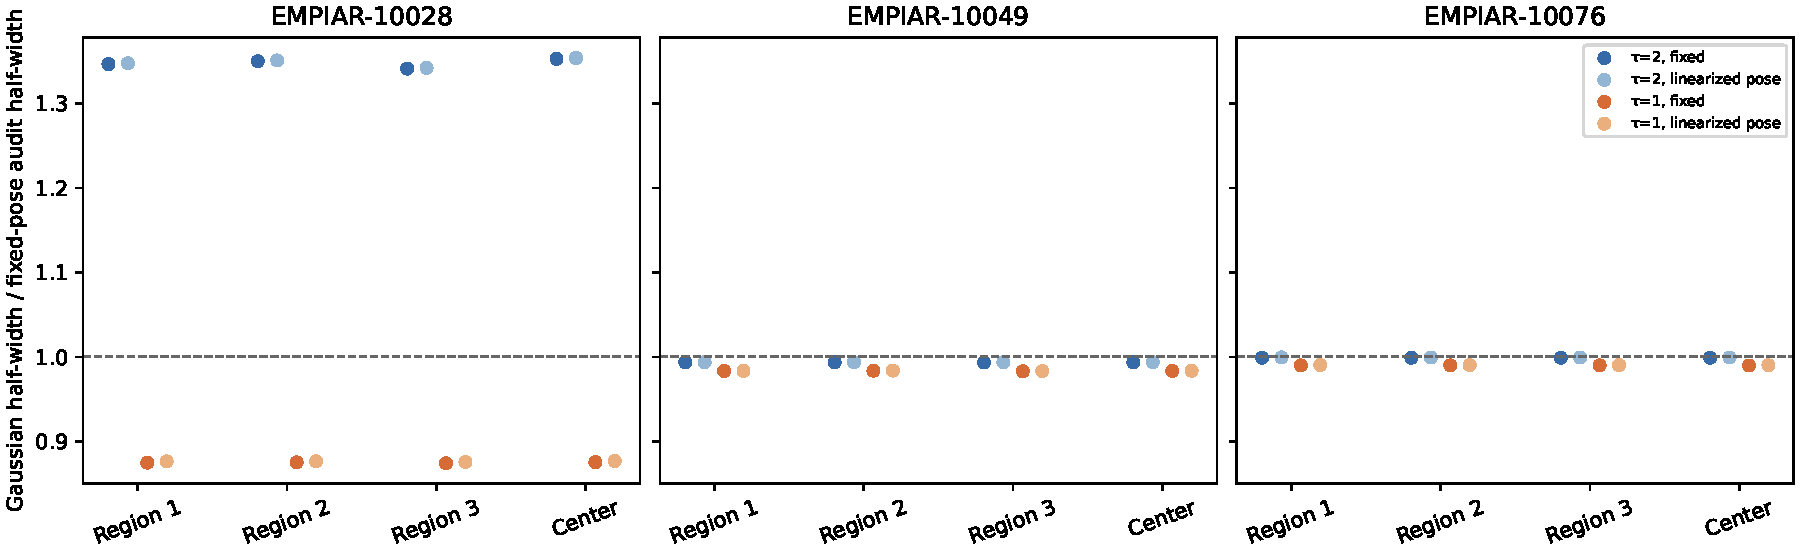
\includegraphics[width=\textwidth]{figures/continuous-gaussian-v2.pdf}
\caption{All twelve locked features and four continuous Gaussian comparisons.
The dashed line denotes the original fixed-pose audit width. Matched prior
scale $\tau=2$ gives near-equal widths on two stacks; its 10028 widths are
34--35\% larger. The half-scale prior is narrower without the same uniform
class implication. Adding the specified first-order Gaussian pose covariance
has little effect here. Every fit converged.}
\label{fig:matchedgaussian}
\end{figure*}
The three complete setup-and-fit runs take 518, 384 and 373 seconds,
respectively, on the authorized Mac under concurrent load. The process peak
resident memory is 6.08 GB; this is a cumulative process high-water mark,
not a fresh per-geometry memory measurement. All relative CG residuals are
at most $9.61\times10^{-11}$. The original rank-1,024 failures are separate
from these 48 successful numerical fits.
}{}
\begin{table}[t]
\centering\small
\caption{Minimum fixed-pose uniform class coverage across four targets, at nominal $1-.05/12=.995833$. Columns separate the prior scale and fixed/linearized covariance weights. These are analytic class minima, not coverage on a selected generator.}
\label{tab:gpclass}
\begin{tabular}{lrrrr}\toprule
Stack & $2$, fixed & $2$, linear & $1$, fixed & $1$, linear \\\midrule
10028 & 0.999930 & 0.999931 & 0.979915 & 0.980143 \\
10049 & 0.995836 & 0.995842 & 0.994882 & 0.994891 \\
10076 & 0.995840 & 0.995851 & 0.995363 & 0.995375 \\
\bottomrule\end{tabular}\end{table}

At prior scale $B/2$, class-worst-case coverage falls below nominal on all
three stacks, although coverage of the selected simulation generators is
favorable. At scale $B$, all 24 class minima exceed .995836. This distinction
prevents treating coverage of benign generators as a uniform class result.

\subsection{Local-pose refitting study}
The calibration seed root is 261001; the test root is 261002. Each is
combined with dataset identifier and replicate index using NumPy's seed
sequence. Calibration contains 128 datasets per geometry; testing has
exactly 200. New alignment noise, inference noise and local initialization
are independently drawn for each replicate. Templates, truth and acquisition
geometry remain fixed. All templates, targets, methods and image controls
within that replicate are paired, not independent observations.

The optimizer uses the frozen ten-iteration Gauss--Newton procedure and its
unchanged step/search constraints. Oracle-template and independent-pilot
fits share the noisy alignment images and initialization. Pose search is
local around near-truth initialization; we do not claim global orientation
discovery. Estimated translations dephase both observation controls and
estimated rotations define a new Fourier Gram. Every interval weight is
recomputed. The affine inference pilot remains the independent pilot even
when the alignment template is oracle truth. Thus the oracle control
isolates reference quality for alignment, not an oracle density estimator.

Fixed-audit weights minimize the sum objective with 100 maximum iterations
and relative-gap target .005. Gaussian fits use relative CG tolerance
$10^{-10}$ and at most 2,000 iterations. Quadrature order is 40 and
preconditioner rank 1,024. Local-Gaussian pose SDs are calibration RMS errors
per coordinate, without removing mean error. These differ from the fixed
$1^\circ$/.5\,\AA\ values in the separate radius-12 comparison.

All nine procedures, both targets, both templates and both image controls
give 72 interval cells per replicate. The first five procedures retain raw
and no-data-selected results; all four Gaussian procedures are reported
raw. Selection compares widths using the fitted design, not the inference
value. When the no-data interval wins, both center and width switch to the
pilot/class interval. It can obtain coverage with no sign information, so
fallback rate and raw outcomes must accompany selected coverage.

Every attempted replicate writes a JSON and arrays, including partial
arrays and exception text on failure. Failed trials remain in the planned
denominator of 200. A completed replicate must contain all 72 unique cells.
Summaries require all 200 attempts and recheck hashes of every JSON, array
and calibration input. Exact binomial 95\% intervals quantify Monte Carlo
uncertainty separately for each procedure; they are not simultaneous
confidence bands over all displayed comparisons. Width summaries use the
available outcomes and report their count. Paired image-control discordance
counts and center differences are retained. Empirical cross-particle
correlations and mean errors are unconditional diagnostics, not tests that
establish conditional-on-design centering.
All 600 datasets and 12,000 solves complete. The total recorded test runtime is 19,584 seconds; peak resident memory is below .681 GB per process. All 216 raw/selected coverage fractions are one. The selected pose intervals use no inference information, so their perfect observed coverage is not an informativeness result. All paired coverage discordance counts are zero. The no-data reference is itself conditional on the supplied pilot-centered class; relative width is not biological resolution.

The final pose errors are substantially larger than the near-truth initialization: rotation RMS medians span 11.990--18.481 degrees and shift medians 6.617--9.282\,\AA. Calibration radii are determined by these same poor local-fitting dynamics. The post-outcome arithmetic remainder decomposition retains all 2,400 template/target fits and does not change an interval or scientific parameter. Minimum and maximum nonlinear-remainder fractions of the raw mixed-zero width are .993056 and .995307. The detailed records include all pose errors, unconditional dependence diagnostics, centers, absolute widths, widths relative to estimates and paired differences.
All 216 detailed coverage, fallback and sign-exclusion rows and both heat maps remain in the machine-readable release. Since every coverage entry is one and every pose fallback entry is one, the compact main table reports their common outcome without repeating three pages of identical entries.
\begin{table*}[t]
\centering\footnotesize
\caption{Post hoc audit-weight diagnostics. Each pair is same-image / independent-image; every cell has 200 paired trials. RMSE is divided by the fixed pilot absolute error. The complete release includes all five distinct estimators, all radius choices, and individual Monte Carlo intervals.}
\label{tab:refittingbias}
\begin{tabular}{lllrrr}\toprule
Stack & Pose control & Target & Mean error / SD & Noise-only coverage & RMSE / pilot error \\\midrule
10028 & True poses & center & -0.367 / -0.400 & 0.920 / 0.925 & 0.061 / 0.062 \\
10028 & True poses & contrast & -0.099 / -0.139 & 0.965 / 0.965 & 0.276 / 0.311 \\
10028 & Oracle template & center & -0.258 / -0.539 & 0.925 / 0.895 & 0.056 / 0.069 \\
10028 & Oracle template & contrast & -0.156 / 0.137 & 0.960 / 0.935 & 0.265 / 0.297 \\
10028 & Pilot template & center & -1.177 / -1.266 & 0.815 / 0.750 & 0.085 / 0.092 \\
10028 & Pilot template & contrast & 0.217 / 0.239 & 0.965 / 0.940 & 0.299 / 0.325 \\
10049 & True poses & center & 0.081 / 0.070 & 0.930 / 0.980 & 1.432 / 1.391 \\
10049 & True poses & contrast & 0.198 / 0.194 & 0.930 / 0.955 & 1.029 / 0.999 \\
10049 & Oracle template & center & 0.737 / -0.295 & 0.900 / 0.925 & 1.590 / 1.478 \\
10049 & Oracle template & contrast & -0.128 / 0.656 & 0.950 / 0.895 & 0.757 / 1.018 \\
10049 & Pilot template & center & 0.638 / -0.557 & 0.905 / 0.925 & 1.600 / 1.594 \\
10049 & Pilot template & contrast & 1.007 / 1.349 & 0.860 / 0.720 & 1.127 / 1.350 \\
10076 & True poses & center & -0.282 / -0.173 & 0.920 / 0.960 & 0.343 / 0.314 \\
10076 & True poses & contrast & -0.068 / -0.161 & 0.955 / 0.925 & 0.758 / 0.872 \\
10076 & Oracle template & center & 0.363 / -0.384 & 0.955 / 0.915 & 0.317 / 0.330 \\
10076 & Oracle template & contrast & 0.165 / -0.024 & 0.950 / 0.945 & 0.689 / 0.797 \\
10076 & Pilot template & center & 0.941 / -0.325 & 0.860 / 0.935 & 0.433 / 0.332 \\
10076 & Pilot template & contrast & -0.162 / 0.081 & 0.965 / 0.950 & 0.718 / 0.792 \\
\bottomrule\end{tabular}
\end{table*}


\subsection{Experimental breakdown analysis}
For each fixed estimator, the stored pilot, density-radius coefficient,
pose remainder and noise scale determine a width as $B$ or measurement SD
is varied. The reporting script reconstructs the stored $B=2$ result to
$10^{-9}$ tolerance before solving where the interval first contains zero.
It reports all 96 feature/pose/calibration combinations; it does not refit
weights at each radius. A breakdown of zero means the feature already
fails sign exclusion at zero radius or noise. It is not evidence that the
true density radius is zero.

At one degree, every retained fixed-weight bias bound already exceeds the
observed center at zero measurement SD. At fixed poses, centered-calibration
10028 breakdowns range from 2.877 to 4.868. These sensitivities measure how
far an assumed input can move before a reported conclusion changes; they
do not estimate that input or validate the common-noise law. The inference
centers were known before this analysis. All raw/selected widths,
no-data-fallback flags and registered-reference disagreements remain saved.
\IfFileExists{tables/breakdown-radii.tex}{\begin{table*}[p]
\centering\small
\caption{Density-radius breakdowns for every locked feature and both experimental noise calibrations. Each pair is raw/centered calibration. Zero means sign exclusion already fails at $B=0$; the declared radius is $B=2$. These are fixed-weight sensitivity thresholds, not estimates of the true radius. Every one-degree noise-scale breakdown is zero. Full half-width/center ratios, noise thresholds and fallback flags are retained in the all-case CSV.}
\begin{tabular}{llrrrr}
\toprule
Stack & Feature & Fixed poses & Shifts only & One degree & Two degrees \\
\midrule
10028 & Region 1 & 3.447/4.832 & 0.516/0.757 & 0.000/0.000 & 0.000/0.000 \\
10028 & Region 2 & 3.444/4.868 & 0.542/0.807 & 0.000/0.000 & 0.000/0.000 \\
10028 & Region 3 & 1.595/2.877 & 0.187/0.395 & 0.000/0.000 & 0.000/0.000 \\
10028 & Center & 1.612/3.055 & 0.193/0.457 & 0.000/0.000 & 0.000/0.000 \\
\addlinespace
10049 & Region 1 & 0.000/153.172 & 0.000/3.401 & 0.000/0.000 & 0.000/0.000 \\
10049 & Region 2 & 0.000/0.000 & 0.000/0.000 & 0.000/0.000 & 0.000/0.000 \\
10049 & Region 3 & 0.000/0.000 & 0.000/0.000 & 0.000/0.000 & 0.000/0.000 \\
10049 & Center & 0.000/133.654 & 0.000/2.854 & 0.000/0.000 & 0.000/0.000 \\
\addlinespace
10076 & Region 1 & 119.076/186.381 & 7.143/11.239 & 0.000/0.054 & 0.000/0.000 \\
10076 & Region 2 & 68.808/126.048 & 4.158/7.692 & 0.000/0.000 & 0.000/0.000 \\
10076 & Region 3 & 111.064/178.140 & 6.626/10.713 & 0.000/0.016 & 0.000/0.000 \\
10076 & Center & 89.151/161.521 & 5.332/9.752 & 0.000/0.000 & 0.000/0.000 \\
\addlinespace
\bottomrule
\end{tabular}
\end{table*}
}{}

\subsection{Reconstruction baselines and FSC interpretation}
Stock cryoDRGN 4.3.1 homogeneous training uses supplied consensus poses,
three hidden layers of width 256 and batch size eight, separately on both
exposure-group halves of each stack. These are actual neural fits, not
backprojection, but are not ab initio CryoDRGN-AI or uncertainty inference.
Gaussian and voxel ridge fits use those same halves. Held-out image scoring
uses identical particles, 1,410 Fourier pairs per image inside radius 30
of a 64-pixel grid, and the same window/background normalization. Stock
neural training uses its radius-32 loss and per-half global scale, so the
training objectives differ. Tuning-group prediction error selects epochs
60, 50 and 100; two are final available checkpoints and undertraining
remains possible. The development stopping budgets are not preregistered
convergence criteria.
\begin{table*}[t]
\centering
\caption{Frozen additional-exposure prediction: 4,096 particles per dataset from 115, 71 and 185 source groups absent from development. Models and cohort were locked before image access. Lower normalized prediction MSE is better. Supplied consensus poses/CTFs remain conditional; this does not measure unknown density coverage.}
\label{tab:freshprediction}
\begin{tabular}{lrrr}\toprule
EMPIAR & Gaussian & Voxel & Neural \\\midrule
10028 & 0.835319 & 0.841379 & 0.829369 \\
10049 & 0.931579 & 0.932359 & 0.930739 \\
10076 & 0.874799 & 0.879078 & 0.868657 \\
\bottomrule\end{tabular}
\medskip

\begin{tabular}{llrl}\toprule
EMPIAR & Comparator minus neural & NMSE difference & Adjusted percentile interval \\\midrule
10028 & Gaussian & 0.005950 & [0.004995, 0.006932] \\
10028 & Voxel & 0.012011 & [0.010695, 0.013356] \\
10049 & Gaussian & 0.000840 & [0.000659, 0.001023] \\
10049 & Voxel & 0.001620 & [0.001366, 0.001875] \\
10076 & Gaussian & 0.006143 & [0.005686, 0.006593] \\
10076 & Voxel & 0.010421 & [0.009792, 0.011038] \\
\bottomrule\end{tabular}
\par\small{All six prespecified paired differences are shown. Intervals use 10,000 whole-exposure bootstrap resamples and a Bonferroni adjustment for six contrasts (99.1667\% marginal percentile intervals). This is a bootstrap approximation, not a finite-sample coverage theorem. No model selection uses these outcomes.}
\end{table*}


RELION 5.0.1 learns poses on all three stacks using a common prescribed
initialization/refinement protocol, with exposure-half labels verified.
Wall-limited initial attempts and separately declared continuations remain
available. No checkpoint is chosen by reference FSC. Native half FSC is
computed before map registration, unmasked, with the coupled low-frequency
region displayed: RELION joins halves below $1/40$\,\AA$^{-1}$.
Cross-method and external-reference FSC use the fixed pilot-only frame/hand
transform, retaining interpolation and registration limits. All native and
registered curves are provided, including poor agreement.

\begin{figure*}[t]
\centering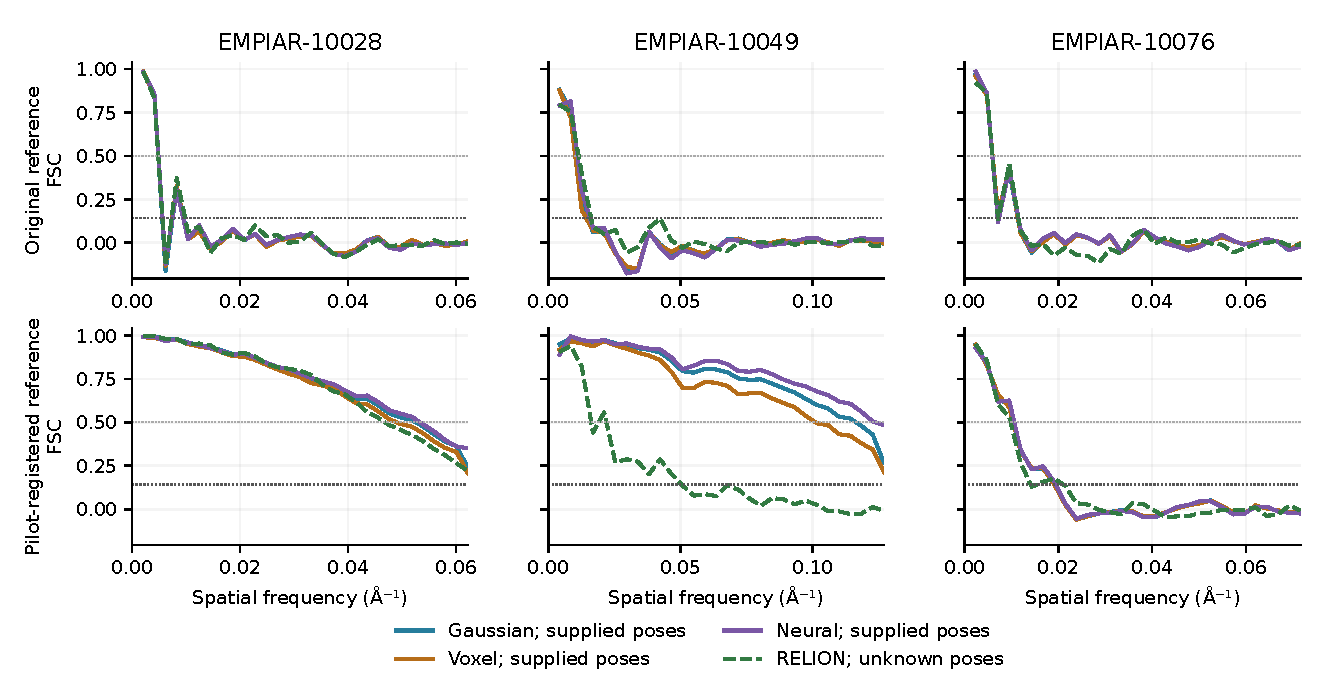
\includegraphics[width=\textwidth]{figures/registered-reconstruction-fsc.pdf}
\caption{All twelve reconstruction method/stack comparisons against original
and pilot-registered references; dotted lines mark FSC 0.5 and 0.143.
Gaussian, voxel and neural fits use supplied poses; RELION estimates poses.
The old pilot alone determines registration. Agreement includes preprocessing,
interpolation and frame dependence. Censored crossings are not measured
resolutions. The 10076 Class A reference is not truth for its heterogeneous
consensus, and none of these curves measures interval coverage.}
\label{fig:registeredfsc}
\end{figure*}

For 10049, native FSC crosses .5 at 22.73\,\AA\ and .143 at
18.95\,\AA. For 10076 these crossings are 24.73 and 15.92\,\AA.
The registered-reference mean FSCs are .702, .202 and .122 for 10028,
10049 and 10076. Mean FSC is a descriptive average over the recorded shells,
not a resolution measure. The heterogeneous third stack and state-specific
reference limit interpretation. Half-map agreement above a threshold
through the sampled band is reported as censored at that limit, not an
observed threshold crossing. Algorithmic convergence also does not establish
structural accuracy.

Original-code CryoLike likelihood scoring and held-out prediction provide
additional image-fit context. A likelihood or FSC is not a confidence
interval for the unknown true feature; we do not use those methods as if
they promised such coverage. Conversely, weak reconstruction agreement is
not hidden by reporting only an uncertainty diagnostic.
Figures~\ref{fig:slices10028}--\ref{fig:slices10076} show every method
in the same three central planes, with display normalization stated explicitly.
\begin{figure*}[p]
\centering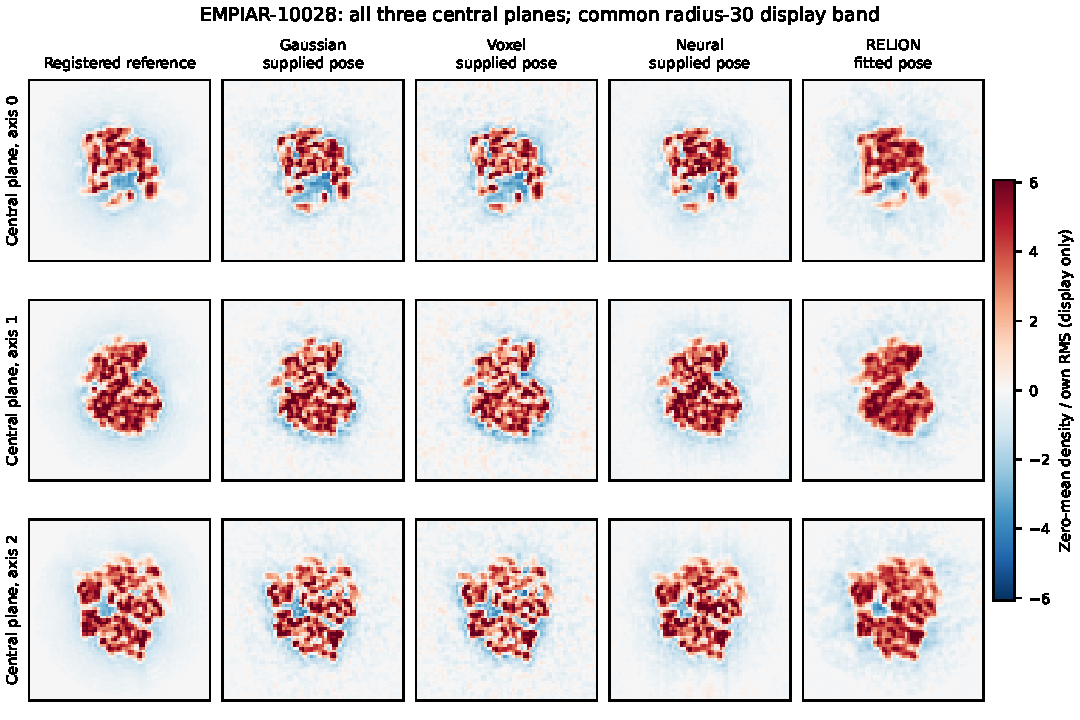
\includegraphics[width=\textwidth]{figures/reconstruction-slices-10028.pdf}
\caption{EMPIAR-10028: all three central planes of the registered reference and four existing reconstructions. Each square spans 482.4\,\AA. The display removes DC, retains a common radius-30 Fourier band, and divides each map by its own volumetric RMS; a pooled 99.5th-percentile absolute value fixes the common symmetric color range. This display normalization hides amplitude differences and is not used for FSC or intervals. Views are fixed array planes, not selected for agreement. Gaussian, voxel and neural estimates average the locked halves; RELION uses its previously evaluated map. Registration is pilot-derived. The 10076 reference represents Class A, not the heterogeneous consensus.}
\label{fig:slices10028}
\end{figure*}
\begin{figure*}[p]
\centering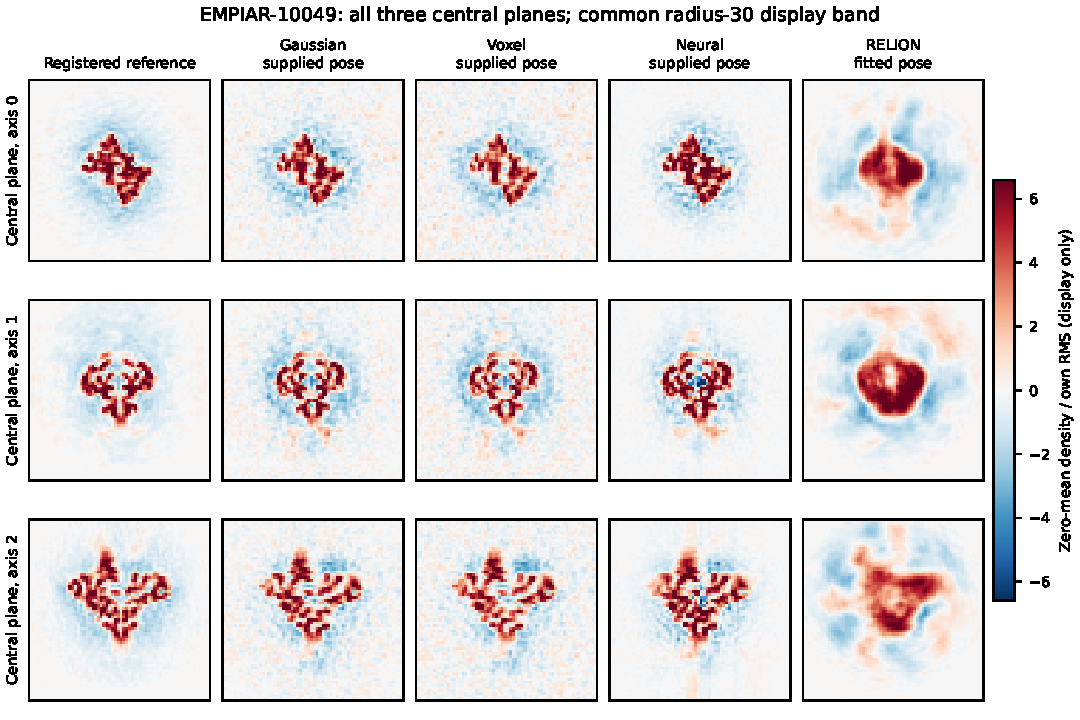
\includegraphics[width=\textwidth]{figures/reconstruction-slices-10049.pdf}
\caption{EMPIAR-10049: all three central planes of the registered reference and four existing reconstructions. Each square spans 236.16\,\AA. The display removes DC, retains a common radius-30 Fourier band, and divides each map by its own volumetric RMS; a pooled 99.5th-percentile absolute value fixes the common symmetric color range. This display normalization hides amplitude differences and is not used for FSC or intervals. Views are fixed array planes, not selected for agreement. Gaussian, voxel and neural estimates average the locked halves; RELION uses its previously evaluated map. Registration is pilot-derived. The 10076 reference represents Class A, not the heterogeneous consensus.}
\label{fig:slices10049}
\end{figure*}
\begin{figure*}[p]
\centering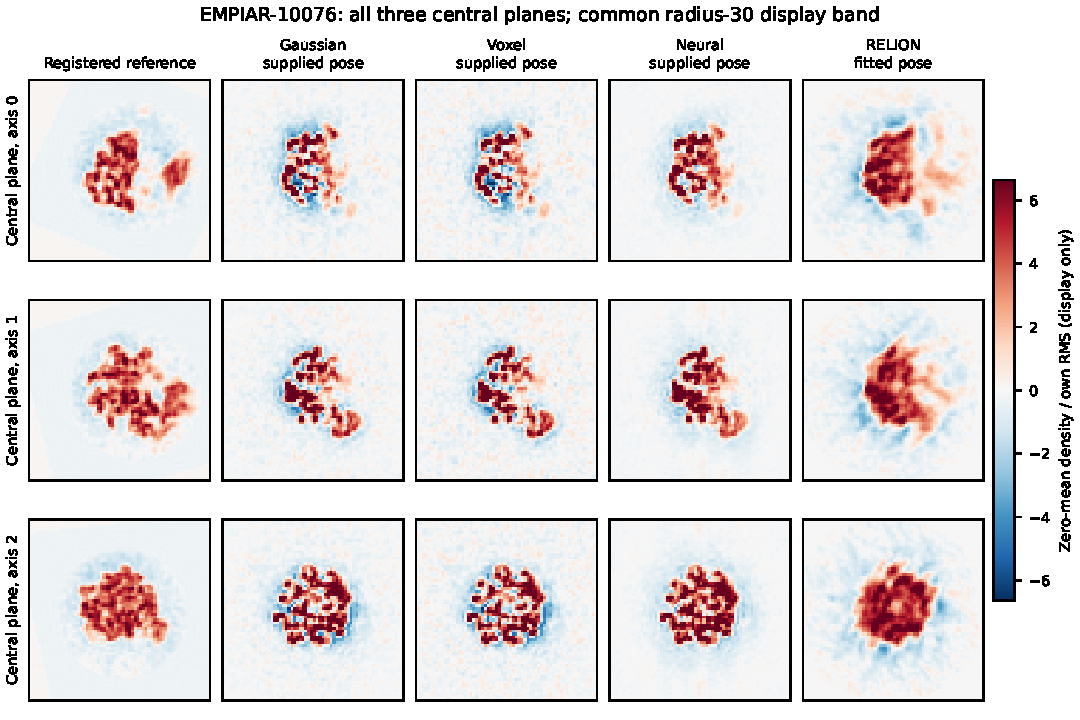
\includegraphics[width=\textwidth]{figures/reconstruction-slices-10076.pdf}
\caption{EMPIAR-10076: all three central planes of the registered reference and four existing reconstructions. Each square spans 419.2\,\AA. The display removes DC, retains a common radius-30 Fourier band, and divides each map by its own volumetric RMS; a pooled 99.5th-percentile absolute value fixes the common symmetric color range. This display normalization hides amplitude differences and is not used for FSC or intervals. Views are fixed array planes, not selected for agreement. Gaussian, voxel and neural estimates average the locked halves; RELION uses its previously evaluated map. Registration is pilot-derived. The 10076 reference represents Class A, not the heterogeneous consensus.}
\label{fig:slices10076}
\end{figure*}


\subsection{Raw-movie feasibility and remaining dependence}
A separately declared acquisition pilot downloaded one EMPIAR-10028 movie,
\texttt{Micrographs\_part2/004\_movie.mrcs}, with 16 frames of
$4096\times4096$ float32 pixels. The source-group mapping is supported by
archive counts, acquisition date and nearby coordinates, but the deposited
autopicks differ from final recentered coordinates. It is not labeled a
fully verified new confirmatory cohort. Its completed analysis is restricted
to all-frame acquisition statistics, a fixed patch grid, frame-difference
spectra/correlations and unaligned odd/even sums. Differences can contain
motion, dose signal and detector effects; they are not automatically pure
noise or proof of frame independence. No density intervals result from this
pilot. Any subsequent motion, picking, CTF or alignment pipeline requires
its own declared processing graph and cannot claim independent inference
noise while silently reusing full-movie-derived quantities.

All sixteen frames, 512 fixed patch differences and 1,792 cross-pair
correlations were retained. Median horizontal and vertical neighbor
correlations are .657 and .658; the 5th--95th percentiles of disjoint
difference correlation are $-.00780$ to $.00866$. Frame means span
2052.53--2060.28 in deposited pixel units. The difference fields are spatially
correlated; these statistics do not separate detector noise from residual
signal. Small temporal correlations do not establish independence or a
transferable covariance.
The interrupted download and verified byte-range recovery are preserved;
they did not change the predeclared movie or diagnostics.
\begin{table*}[t]
\centering\small
\caption{Predeclared acquisition diagnostics from one raw 10028 movie. Difference statistics use every one of 512 patch/pair combinations; disjoint-pair correlations use all 1,792 comparisons. Quantiles are descriptive across dependent summaries, not independent-replicate confidence intervals.}
\begin{tabular}{lrrrrr}
\toprule
Statistic & Minimum & 5th percentile & Median & 95th percentile & Maximum \\
\midrule
Difference SD & 341.7 & 351.2 & 357.7 & 370.3 & 402.5 \\
Horizontal neighbor correlation & 0.6455 & 0.6496 & 0.6569 & 0.6641 & 0.6844 \\
Vertical neighbor correlation & 0.6463 & 0.6522 & 0.6583 & 0.6662 & 0.6862 \\
Disjoint-difference correlation & -0.01856 & -0.007798 & 0.0006576 & 0.008661 & 0.01639 \\
\bottomrule
\end{tabular}
\end{table*}


% Reset the two-column page height after the flushed double-column floats.
\onecolumn
\twocolumn
\section{Uncertainty Targets in the Recent Literature}\label{app:survey}
The retrieval ledger contains 16,969 deduplicated broad-search records, mostly applications and not individually screened methods. The following distinctions guide baseline selection. They do not rank methods that solve different problems on one inappropriate score. The accompanying dated survey has 126 curated candidates across reconstruction, poses, heterogeneity, map validation, atomic ensembles and general inverse inference; its source manifest distinguishes retrieved material from targeted critical reading and inaccessible full text. This is a scoped critical survey rather than a claim to have exhaustively reviewed all cryo-EM applications. Versioned preprints are identified separately from published articles.

\paragraph{Additional local and atomic validation.} The recent Gold-standard local toolbox compares half-map phase and amplitude, with explicit independent-noise assumptions in its SNR derivation \citep{goldlocal2026}. EMMIVox combines molecular force fields, map likelihoods and half-map-informed uncertainty for atomic refinement \citep{emmivox2024}. Neither output is the fixed raw-particle density functional studied here.

\paragraph{Distributional inverse stability.} The recent revision of
\citet{stochastic2026} separates image-distribution discrepancy from latent
Wasserstein error under assumed local stability. Its observability inequality
bounds stability above, not below; it does not certify experimental coverage.
A correctly specified Gaussian-mixture baseline wins its matched synthetic
comparison, illustrating the importance of retaining favorable baselines.

\paragraph{Direct statistical uncertainty prior art.} The probabilistic Fourier-slice model of \citet{ullrich2020} is a close reconstruction-uncertainty comparator and explicitly recognizes model bias. Joint likelihood soft modes \citep{rangan2024} expose pose--density ambiguities. \citet{lai2023} connect empirical Bayes and sequential MCMC filtering to dynamic image reconstruction, including scalar confidence sets and hybrid resampling. Their approximate fitted-family resampling and posterior computations differ from the present uniform conditional bounded-class statement; they cannot be dismissed as deterministic reconstruction methods. Neither general bias-aware inference nor the distinction between posterior variance and model error originates here.

\paragraph{Latent orientations and moment validation.}
Nonuniform moment recovery has explicit bandlimit and genericity conditions;
numerical Jacobian ranks in unknown-law cases differ from exact uniqueness
proofs \citep{sharon2020}. SubspaceMoM compresses moments to jointly recover
structure and viewing laws, with its principal reconstruction tests on
synthetic CTF-corrupted images \citep{subspacemom2026}.
High-noise Fisher stratification for marginalized orbit likelihoods assumes
Haar rotations, generic signals and projected identifiability conditions
\citep{fan2024}; it is not per-particle pose calibration.
Moment-based structural comparison also profiles a viewing-law expansion
\citep{momentmetrics2024}. Its 10076 example uses separate states and deposited
shifts, with remaining acquisition effects and limited close-state discrimination.
These are substantive alternatives to conditional local-pose analysis, without
establishing the same finite-sample feature guarantee.

Adjacent radiative CT work also separates analytic Gaussian uncertainty from shared reconstruction error and distinguishes foreground evaluation from whole-volume scores \citep{zhao2026radiative}. Its density-moment formulas and validation distinctions further constrain novelty claims; its acquisition and estimands differ from cryo-EM.

Bayes' Rays uses post-hoc displacement uncertainty for a frozen NeRF, with a diagonal curvature approximation \citep{goli2024}. Its spatial target differs from an additive density interval. The dynamic extension proposed in \citet[Section 5.2]{patel2025thesis} is explicitly future work, with cryo-EM as an intended application; we do not treat that proposal as an experimentally validated density guarantee.

\paragraph{Pose inference versus pose confidence.} Posterior-averaged orientation estimation \citep{bayespose2026} and probabilistic orientation search in SIMPLE \citep{simple2025} improve pose estimation through different statistical or optimization constructions. Neither an orientation distribution nor a stochastic search neighborhood should be relabeled a calibrated per-particle confidence ball without verifying its guarantee. Our prescribed local balls avoid that claim, but consequently do not solve practical pose calibration.

Cryo-forum uses quaternion-distribution dispersion for error ranking and filtering \citep{cryoforum2023}. ARCHER learns reference-conditioned pose scores and evaluates cross-specimen transfer and junk rejection \citep{archer2026}. CESPED standardizes experimental poses obtained by refinement, and explicitly acknowledges uncertainty in those labels \citep{cesped2024}. CryoPARES transfers alignments between related experiments \citep{cryopares2026}; CryoFastAR combines multiview pose prediction, synthetic training and experimental fine-tuning \citep{cryofastar2025}. These approaches address efficiency and different transfer settings. Their quality scores and angular errors cannot supply a uniform maximum-error radius for every particle in a new stack. The $0.1^\circ$ and $0.5^\circ$ budgets in our frozen study are sensitivity settings, not experimentally established alignment accuracy.

\paragraph{Physical heterogeneity versus estimation error.} RECOVAR estimates covariance and uses kernel regression to account for noisy latent coordinates \citep{recovar2025}. DynaMight and 3DFlex represent motion \citep{dynamight2024,flex2023}. Particle-counting work explicitly studies when assignments misestimate state populations \citep{counting2026}. These motivate separate tests of population recovery, structural variation and uncertainty in a homogeneous density. The present bounded-density target covers only the last. CryoDRGN-AI addresses joint ab initio reconstruction \citep{drgnai2025}; fixed-pose homogeneous training does not reproduce that task.

DynaMight's held-out deformation disagreement and independent-half training assess motion errors; 3DFlex separates lower-frequency motion training from higher-frequency reconstruction validation. Their protocols must be examined at the level of shared components and evaluated frequencies. \citet{mattingly2026} study how the image model limits learnable conformational populations, using information-based selection of ensemble granularity. That prior-averaged population target differs from our fixed homogeneous density functional. CryoBench likewise distinguishes representation learning, conformation assignment and volume recovery with several reference-based FSC metrics \citep{cryobench2025}. Our simulations posit one density per acquisition geometry; the actual stacks need not be homogeneous. In particular, the assembly-intermediate mixture in EMPIAR-10076 does not validate our shared-density assumption.

\paragraph{Map validation and learned priors.} False-discovery confidence maps test density significance against a noise reference \citep{beckers2019}. Directional resolution measures acquisition anisotropy \citep{monodir2020}; independent-particle tests assess map fit \citep{independent2020}. Bias/variance analyses explain why validation requires more than internal agreement \citep{sorzano2022}. Blush introduces learned reconstruction regularization \citep{blush2024}, while LocScale-2.0 attaches confidence to enhancement relative to its stated proxy \citep{locscale2026}. Compressed-image recovery with cryoSENSE targets acquisition fidelity rather than density-confidence coverage \citep{cryosense2026}. Matched evaluations must retain these targets. A sharper-looking map or a significant positive voxel is not itself a bound on error relative to unknown density.

Fixed-candidate ensemble analysis also separates discretization bias, statistical variability and early stopping \citep{mordant2026}. Its simplified known-likelihood population problem differs from spatial density reconstruction with uncertain poses; it does not calibrate the nuisance bounds used here.

CryoRes predicts local resolution using deposited and algorithm-derived training labels \citep{cryores2023}. Such supervision inherits the meaning of those labels; it does not transform a resolution score into a confidence interval. Similarly, held-out image prediction measures agreement with new observations, and can remain favorable when two reconstructions share unsupported density directions. Ground-truth simulation, new-exposure prediction, directional diagnostics and independent structural evidence therefore complement one another.

\paragraph{Invariant compression and thermodynamic targets.} Moment-based posterior sampling conditions a learned prior on shift-invariant power spectra in one-dimensional orbit recovery \citep{janson2025}. Compression discards phase information, so posterior concentration can rely on the prior. Separately, cryoTWIN/PaStEL targets conformational free energies under sampling, pose and equilibrium assumptions \citep{cryotwin2026}. Neither problem is equivalent to our shared-density feature interval.

\paragraph{Atomic ensembles and independent modalities.} Experiment-guided AlphaFold3 conditions structural generation on reconstructed ESP maps and other measurements \citep{guidedaf32026}. Its atomic-ensemble target differs from raw-particle density inference. The multimodal examples also illustrate why improved map agreement need not imply improved fit to a separate measurement modality. Independent evidence is relevant to assessing structural interpretations that the density measurements alone leave ambiguous.

\paragraph{Coordinate-error conformal prediction.} CalPro calibrates protein-coordinate error scores at an exchangeable-protein level \citep{calpro2026}. Its atomic target and calibration unit differ from a fixed density feature inferred from noisy projections. We do not interpret a calibrated protein-average score as simultaneous residue coverage or as experimental-density coverage.

\paragraph{Simultaneous inverse inference.} Constrained test-inversion methods already address joint confidence regions for multiple functionals \citep{batlle2025}. A single data-consistency region can support simultaneous projections, whereas separately calibrated marginal intervals generally require an appropriate correction. Our present scalar-target theorem is not a new general framework for simultaneous inference, and a colored map of marginal intervals must not be presented as simultaneous coverage.

\paragraph{Conformal calibration and its sampling unit.} Posterior-variance calibration can provide error bounds even when a posterior sampler is approximate \citep{narnhofer2024}; its theorem uses independent identically distributed signal--observation pairs and conditions on a variance bin. QUTCC learns quantile-dependent image predictions and calibrates marginal pixel errors from paired reference images \citep{qutcc2026}. These methods can be useful without our fixed-signal radius assumption, but require a calibration population with the stated sampling relationship to deployment. Voxels or noise draws from one molecule are not automatically independent calibration molecules. Neither marginal population coverage nor variance-bin coverage is the same as coverage uniformly over every density in a specified class.

\paragraph{Prior-assisted alignment and atomic refinement.} CryoPROS uses generated auxiliary particles for pose correction, with template-variation and noise-only controls \citep{cryopros2025}. Such tests address model bias without calibrating experimental pose confidence regions. CoCoFold fine-tunes AlphaFold against particle images using a Gaussian-mixture forward model and supplied poses/CTFs \citep{cocofold2026}. Its pose-perturbation checks support a sensitivity comparison, not a density-coverage guarantee. Both motivate independent validation of prior-assisted inference; neither is a matched density-functional uncertainty baseline here.

\paragraph{Open questions suggested by the survey.} Particularly consequential gaps are absolute pose-confidence calibration under reference error; uncertainty in conformational populations when candidate structures are imperfect; validation of detail introduced by learned priors using independent particles; and uncertainty propagation through CTF fitting, image preprocessing, alignment and atomic interpretation. Acquisition chosen for a specific structural feature is another possible application of adjoint sensitivity. These are directions inferred from the literature, not priority claims or completed capabilities of this implementation. The present continuous audit addresses representation exclusion under stated nuisance assumptions; solving those assumptions empirically remains distinct work.


\paragraph{Alignment attenuation and conditioning.} Classical alignment-error envelopes include orientation, location and other imaging errors \citep{jensen2001}. Cross-validation against overfitting and noise correlation in three-dimensional alignment is also established \citep{shaikh2003}. For these two historical papers our reading is limited to the primary author abstracts; we do not claim to have verified their full derivations. SIMPLE's shared orientation-table updates \citep{simple2025} illustrate that particle-wise local fits against a frozen template are not the same stochastic procedure as a full reconstruction pipeline. The phase control in Appendix~\ref{app:phase} is therefore a diagnostic, not a discovery of alignment-induced bias.

\end{document}
